\chapter{ \toolName の外観と機能}\label{cha:Function}
本章では、本研究で試作したツール\toolName (Mix Visual Regression Test)の外観と機能について説明する。
\par
\toolName は、レイアウトの不具合の発見を支援する、視覚的回帰テスト支援ツールである。

\section{\toolName の前準備}\label{sec:preparation}
\toolName で視覚的回帰テストを行うための前準備について説明する。
\toolName を使用する前提として、開発者が開発初期段階のWebページを作成していると想定する。
また、HTMLコードの変更を行った際に、その変更をWebページに反映しているものとする。
\par
開発者は以下の手順で視覚的回帰テストを行うための前準備を行う。なお、手順1は\toolName 実行コマンド(\ref{sec:test_execution}節で後述)を使用し、手順2は人手で行う。
\begin{enumerate}
    \item 現時点のWebページの画像を取得する
    \item HTMLコードの変更を行う
\end{enumerate}

\section{\toolName による視覚的回帰テスト実行}\label{sec:test_execution}
\toolName は、Python3.9\cite{Python}が動作するテキスト端末上で実行する。
\toolName 実行時のコマンドライン引数によって、視覚的回帰テストを行う対象のWebページのURLを指定する。
\toolName 実行のための書式は、以下である。
\begin{lstlisting}[label=list:command,frame=none,numbers=none,basicstyle={\normalsize \ttfamily \color[gray]{.15}}]
  $ python3 MixVRT.py URL
 \end{lstlisting}
{\tt URL}には、テスト対象とするWebページのURLを指定する。なお、"https://"または"http://"から始まるURLとする。
\toolName は、テスト対象とするWebページのURLを入力として受け取り、Webページの画像とHTMLコードを取得して画像処理とHTMLコード解析を行うことで、
以下に示すPNG形式の画像を出力する。
なお、\toolName 初回実行時は比較対象となるWebページの画像が存在せず視覚的回帰テストを行えないため、Webページの変更前画像のみを出力する。
% 入力としてWebページのURLを受け取り、
% URLからWebページの画像とHTMLコードを取得し、画像処理とHTMLコード解析を行うことで、
% 【TODO:URLからなぜ画像が出るのかについて説明する】
\begin{itemize}
    \item Webページの変更前画像と変更後画像
    \item 画像比較に基づく差分箇所を色付きの枠で囲んで強調表示した、Webページの変更前画像と変更後画像
    \item HTMLの変更に基づく影響箇所を色付きの枠で囲んで強調表示した、Webページの変更前画像と変更後画像
    \item レイアウトの副作用箇所を色付きの枠で強調表示した、Webページの変更前画像と変更後画像
\end{itemize}


\section{\toolName の外観と機能}\label{sec:Appearance}
\toolName の外観を、図\ref{fig: Appearance}に示す。
\begin{figure}[tp]
    \begin{center}
        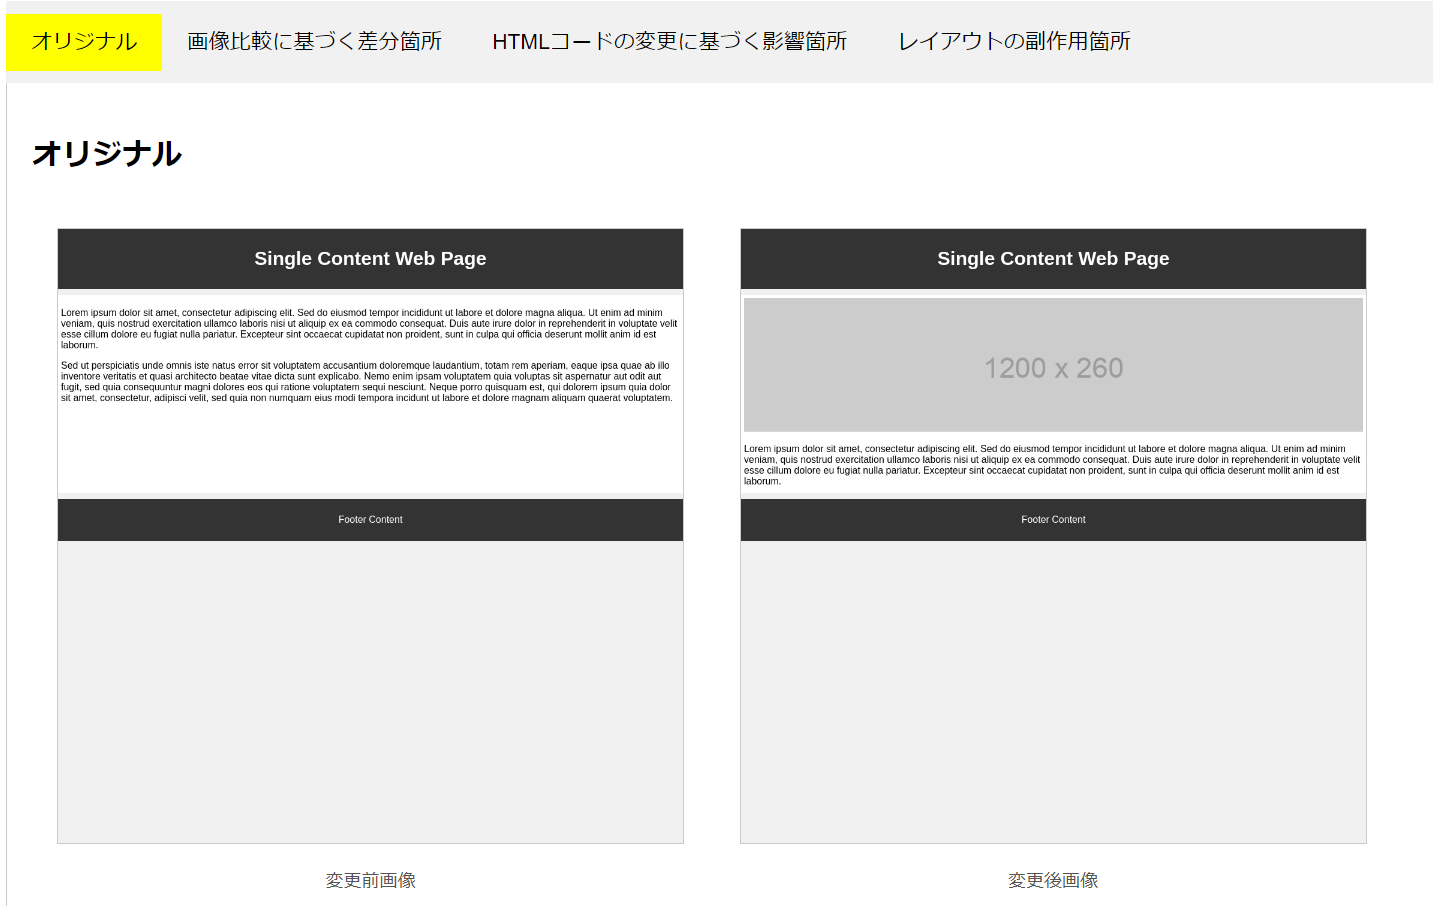
\includegraphics[width=1.0\columnwidth]{image/3_Appearance.png}
        \caption{\toolName の外観}
        \label{fig: Appearance}
    \end{center}
\end{figure}

\toolName は、以下に示す4つのタブからなるタブメニューと各タブに対応した内容を表示するタブコンテンツからなる。
なお、以下の数字は、図\ref{fig: Appearance}の数字と対応している。
\begin{itemize}
    \item[①] タブメニュー
          \begin{itemize}
              \item オリジナル表示タブ
              \item 画像比較に基づく差分箇所表示タブ
              \item HTMLコードの変更に基づく影響箇所表示タブ
              \item レイアウトの副作用箇所表示タブ
          \end{itemize}
    \item[②] タブコンテンツ
\end{itemize}
\par
以降、各タブの外観と機能について説明する。



\section{オリジナル表示タブ}\label{sec:original_tab}
オリジナル表示タブを押すと、Webページの変更前画像と変更後画像を並べて表示する。【DO: del:Webページ,add:並べて】
オリジナル表示タブを押した際の\toolName の画面例を、図\ref{fig: Appearance_original_tab}に示す。
なお、\toolName に一番最初にアクセスした時やリロードした時には、デフォルトでオリジナル表示タブを選択した状態になっている。
このタブでは、Webページの変更前後の画像を目視で確認できる。
\begin{figure}[tp]
    \begin{center}
        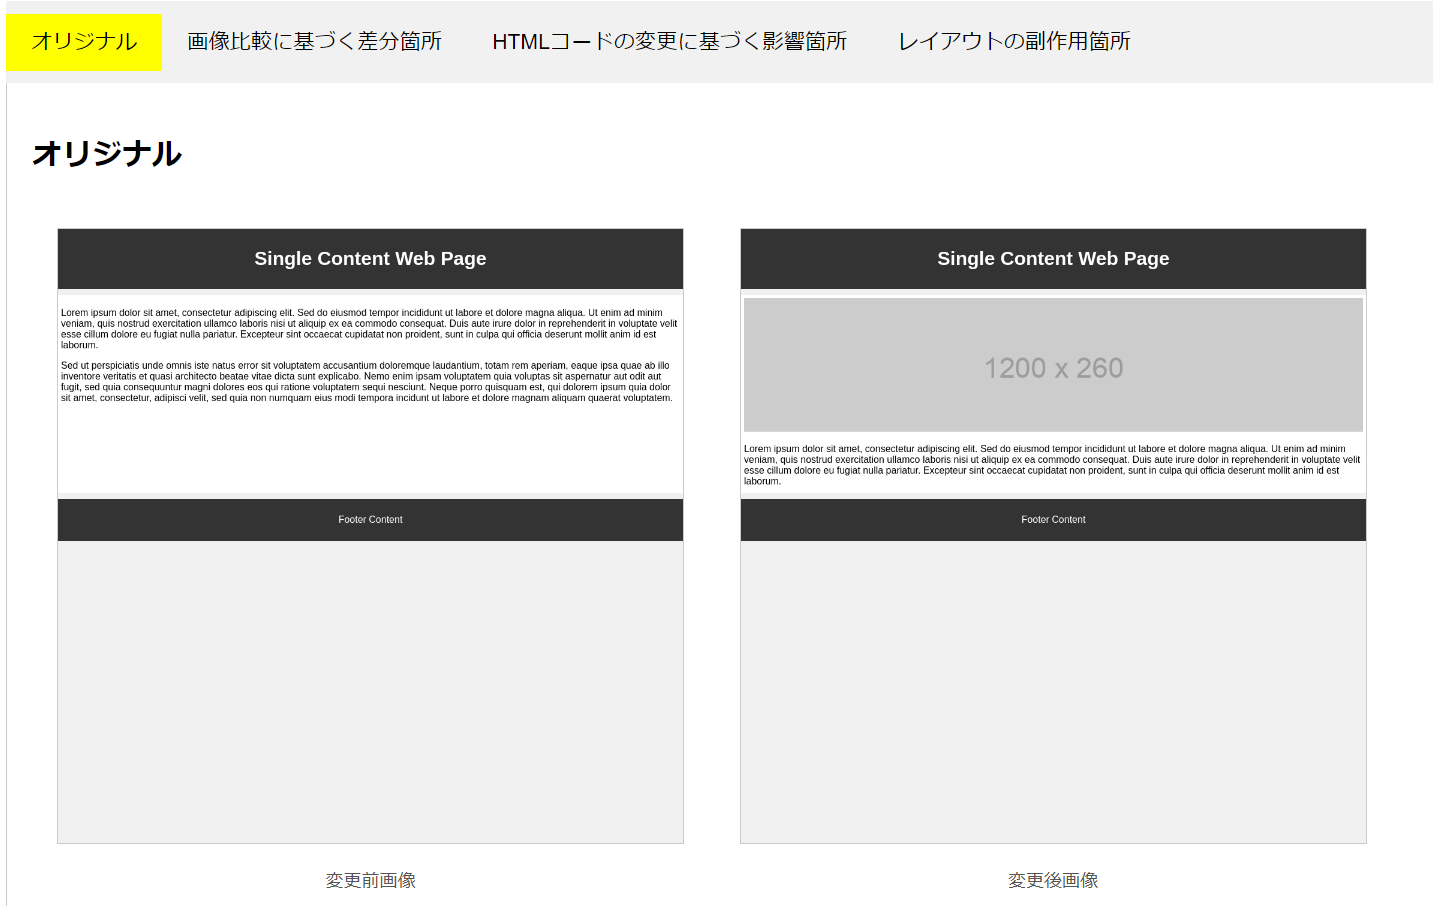
\includegraphics[width=1.0\columnwidth]{image/3_original_tab.png}
        \caption{オリジナル表示タブを押した際の\toolName の画面例}
        \label{fig: Appearance_original_tab}
    \end{center}
\end{figure}



\section{画像比較に基づく差分箇所表示タブ}\label{sec:images_tab}
画像比較に基づく差分箇所表示タブを押すと、画像比較に基づく差分箇所を色付きの枠で囲んで強調表示した、Webページの変更前画像と変更後画像を並べて表示する。【DO: del:Webページ,add:並べて】
画像比較に基づく差分箇所表示タブを押した際の\toolName の画面例を、図\ref{fig: Appearance_images_tab}に示す。
【TODO:差分箇所の説明は3章の初めに書く】ここでの差分箇所とは、変更前後のWebページを比較して、変更前のWebページで削除された箇所と変更後のWebページで追加された箇所を差分箇所と定義する。
削除された箇所は変更前画像上に赤枠で囲んで強調表示し、追加された箇所は変更後画像上に緑枠で囲んで強調表示する。
このタブでは、変更前後のWebページでレイアウトの変更【DO:画素単位での見た目の差分⇒レイアウトの変更】があった箇所を目視で確認できる。
\begin{figure}[tp]
    \begin{center}
        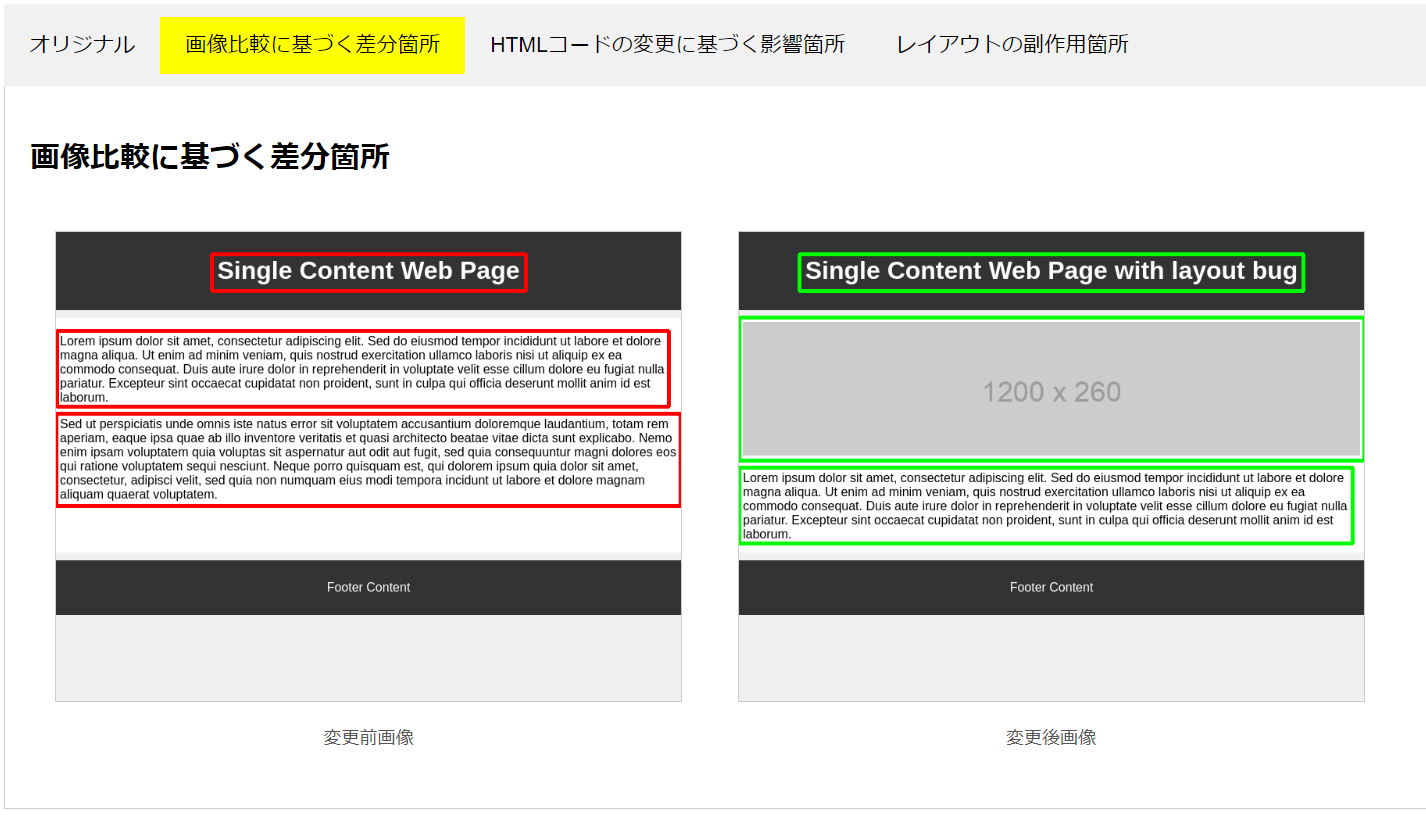
\includegraphics[width=1.0\columnwidth]{image/3_images_tab.png}
        \caption{画像比較に基づく差分箇所表示タブを押した際の\toolName の画面例}
        \label{fig: Appearance_images_tab}
    \end{center}
\end{figure}



\section{HTMLコードの変更に基づく影響箇所表示タブ}\label{sec:html_tab}
HTMLの変更に基づく影響箇所表示タブを押すと、HTMLの変更に基づく影響箇所を色付きの枠で囲んで強調表示した、Webページの変更前画像と変更後画像を並べて表示する。【DO: del:Webページ,add:並べて】
HTMLの変更に基づく影響箇所表示タブを押した際の画面例を、図\ref{fig: Appearance_html_tab}に示す。
【TODO:影響箇所の説明は3章の初めに書く】ここでの影響箇所とは、変更前後のWebページのHTMLコードを比較して、HTMLコードにおけるbody要素内の変更とstyle要素内の変更のどちらか、または両方の影響を受けた画面要素箇所と定義する。
変更前のWebページのHTMLでの影響箇所は変更前画像上に赤枠で囲んで強調表示し、変更後のWebページのHTMLでの影響箇所は変更後画像上に緑枠で囲んで強調表示する。
このタブでは、図\ref{fig: Appearance_images_tab}における差分箇所から、開発者が意図して変更した、または意図せず変更してしまったHTMLコードによる影響箇所を目視で確認できる。
% このタブでは、変更前後のWebページで開発者が意図した、または意図しないHTMLコードの変更による影響箇所を目視で確認できる。
\begin{figure}[tp]
    \begin{center}
        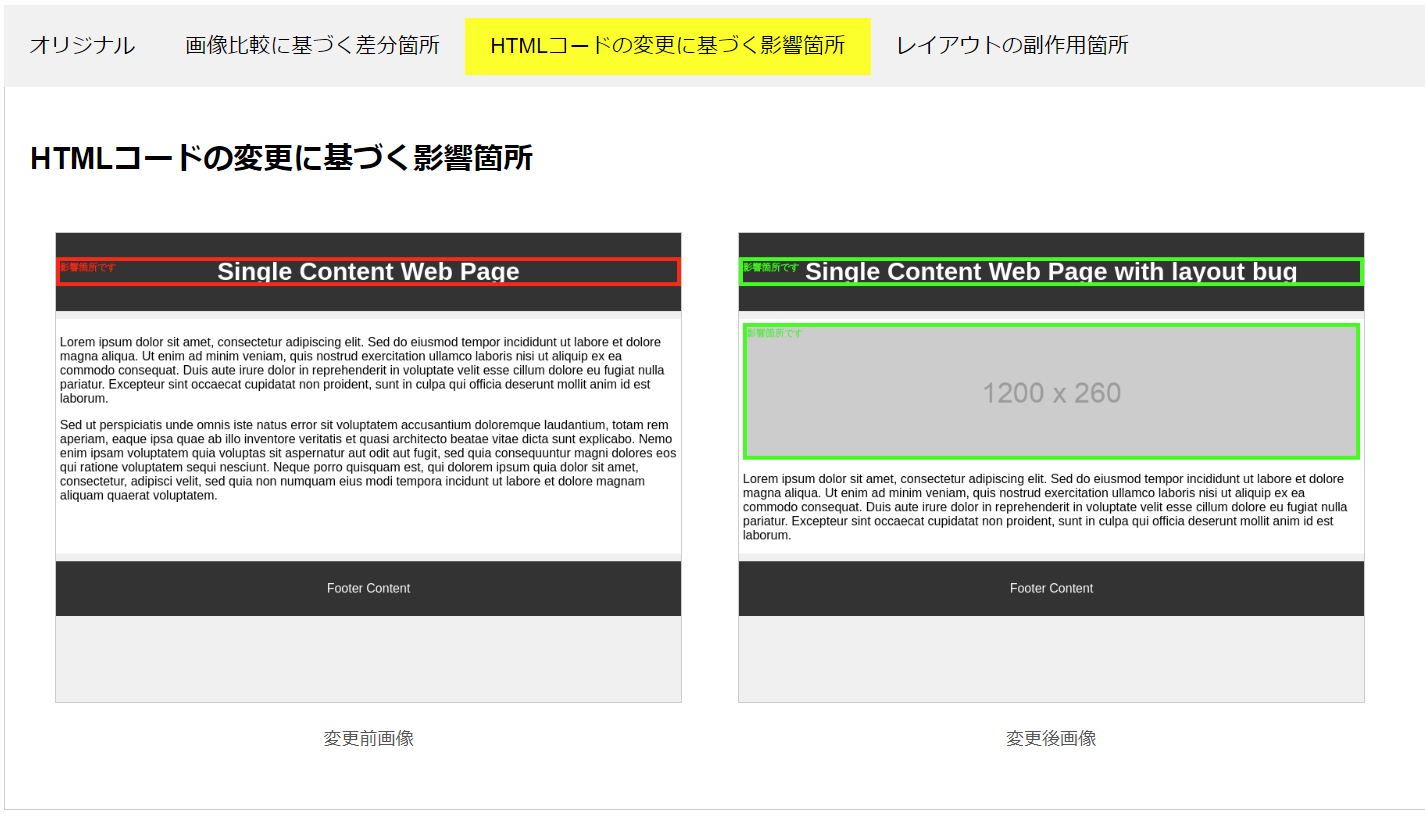
\includegraphics[width=1.0\columnwidth]{image/3_html_tab.png}
        \caption{HTMLコードの変更に基づく影響箇所表示タブを押した際の\toolName の画面例}
        \label{fig: Appearance_html_tab}
    \end{center}
\end{figure}



\section{レイアウトの副作用箇所表示タブ}\label{sec:subeffect_tab}
レイアウトの副作用箇所表示タブを押すと、【TODO: ~と~に基づいての基づいてとは?どう基づいて?】差分箇所と影響箇所に基づいて出力したレイアウトの副作用箇所を色付きの枠で強調表示した、Webページの変更前画像と変更後画像を並べて表示する。【DO: del:Webページ,add:並べて】
レイアウトの副作用箇所表示タブを押した際の画面例を、図\ref{fig: Appearance_subEffect_tab}に示す。
【TODO:レイアウトの副作用箇所の説明は3章の初めに書く。説明の際は本論文での~は~と定義する。という書き方にする】ここでのレイアウトの副作用箇所とは、変更前後のWebページでHTMLコードの変更による影響を受けた画面要素によって、HTMLコードを変更していない画面要素に見た目の変更があった箇所と定義する。
変更前のWebページでのレイアウトの副作用箇所は変更前画像上に赤枠で囲んで強調表示し、変更後のwebページでのレイアウトの副作用箇所は変更後画像上に緑枠で囲んで強調表示する。
このタブでは、図\ref{fig: Appearance_images_tab}における差分箇所から、レイアウトの不具合を含む可能性のある箇所を目視で確認できる。
【TODO:3.4の存在意義とは?】
\par
【実装したいこと:図\ref{fig: Appearance_subEffect_tab}の変更前画像上のある赤枠内の内容と変更後画像上のある緑枠内の内容がほぼ一致した場合に、それらの枠に関してはレイアウトの不具合を含まないレイアウトの副作用とみなして除外する処理】
\par
【実装によって実現できること: レイアウトの不具合箇所のみを目視で確認できる】
\begin{figure}[tp]
    \begin{center}
        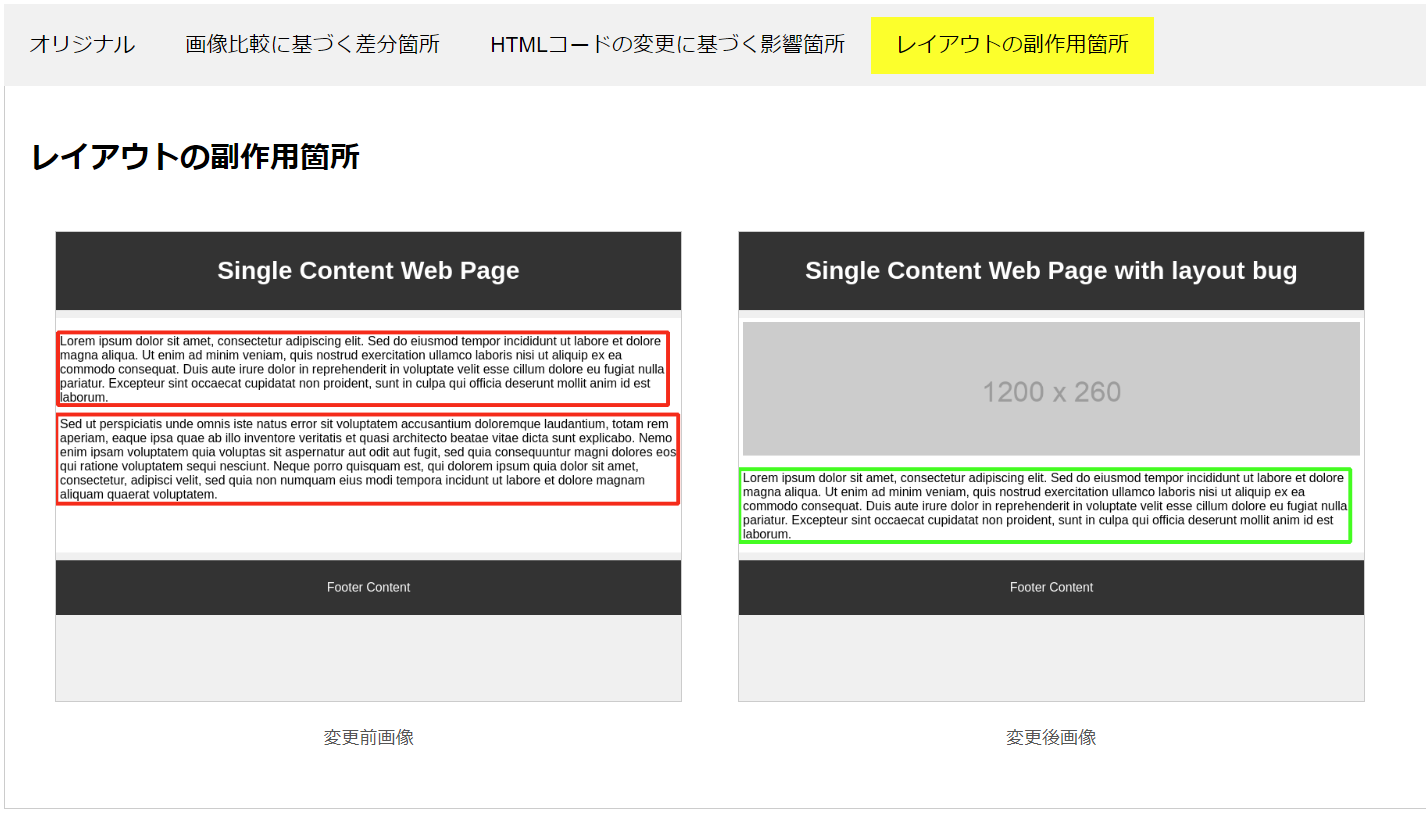
\includegraphics[width=1.0\columnwidth]{image/3_subEffect_tab.png}
        \caption{レイアウトの副作用箇所表示タブを押した際の\toolName の画面例}
        \label{fig: Appearance_subEffect_tab}
    \end{center}
\end{figure}

